\documentclass[11pt]{article}

% template
\usepackage{if69d-template} % Modelo elaborado por Fernando Padilha 

% pacotes
\usepackage[brazil]{babel}
\usepackage[utf8]{inputenc}
\usepackage{graphicx}
\usepackage{amsthm,amsfonts,amsmath}
\usepackage[font=footnotesize,
			labelfont=it,
			labelformat=simple]{subcaption}
\usepackage{url}
\renewcommand\thesubfigure{(\alph{subfigure})}

% capa
\instituicao{Universidade Tecnológica Federal do Paraná -- UTFPR}
\departamento{Departamento Acadêmico de Eletrônica -- DAELN}
\curso{Engenharia Eletrônica} %INSIRA AQUI O NOME DO SEU CURSO
\disciplina{IF69D – Processamento Digital de Imagens}
\semestre{2023.1}
\professor{Gustavo Borba e Humberto Gamba}

\titulo{Algoritmo de processamento de imagens de satélite para análise de área desmatada na Amazônia}

\autor{Danilo Campana Fuchs}{1906755} %INSIRA SUA IDENTIFICAÇÃO
% \autordois{Nome completo}{código} %INSIRA SUA IDENTIFICAÇÃO
\date{Junho 2023} %INSIRA AQUI MÊS E ANO DA ENTREGA


% começo do documento
\begin{document}

\maketitle

\section{Objetivo}

Propor e implementar em MATLAB um algoritmo K-Means para cálculo de área desmatada através da segmentação de floresta e não-floresta na Amazônia, aplicado em imagens de satélite no formato Color Infrared (CIR), da cidade de Candeias do Jamari - Rondônia/BR.


\section{Fundamentação Teórica}

\subsection{Imagens de satélite para monitoramento de desmatamento}

O meio mais eficiente para se monitorar desmatamento em uma floresta de vastas dimensões é através da análise de imagens de satélite. No Brasil, o monitoramento da Amazônia é feito pelo Instituto Nacional de Pesquisas Espaciais (INPE) desde 1988, através do projeto PRODES \cite{inpe:prodes:2022}. Desde 2002, todas as imagens, dados, programas e relatórios do programa são públicos e acessíveis através da plataforma TerraBrasilis \cite{inpe:brasilis:2023}.

Em seus primórdios, o programa utilizava imagens do satélite americano LANDSAT-5/TM que fornecia imagens em 7 diferentes bandas (3 nas faixas visíveis, 4 no infravermelho). Através do programa espacial brasileiro e de parcerias com outras nações, hoje são utilizados imagens de múltiplos satélites brasileiros, sino-brasileiros, indianos, britânicos e americanos, combinando seus espectros para redundância \cite{inpe:prodes:2022}.

% Entre 1988 e 2000, pesquisadores utilizavam imagens do satélite americano LANDSAT-5/TM e efetuavam segmentação manual das imagens de satélite através da análise visual, efetuavam a digitalização dos trechos delineados e sua vetorização para processamento digital (PRODES Analógico), conforme indicado no fluxograma da Figura \ref{fig:prodes_analogico}.

% \begin{figure}[!htb]
% 	\centering
% 	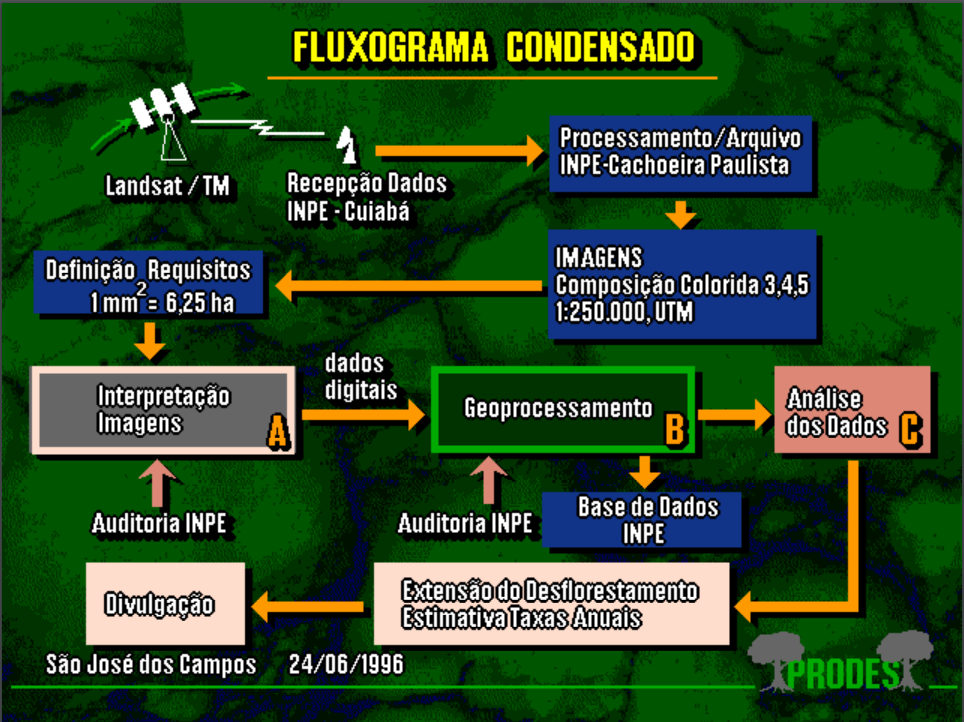
\includegraphics[width=.8\textwidth]{prodes_analogico.png}
% 	\caption{Fluxograma do PRODES Analógico \cite{inpe:analogico:96}}
% 	\label{fig:prodes_analogico}
% \end{figure}

% Entre 2000 e 2005, 


Em 2014, o INPE criou o programa DETER (Sistema de Detecção de Desmatamento em Tempo Real), que fornece relatórios diários ao IBAMA com a localização precisa de novos focos de desmatamento.

Em 2020, o governo da Noruega -- através de seu fundo para combate às mudanças climáticas -- licenciou as imagens das florestas tropicais obtidas mensalmente pela empresa americana Planet Labs PBC \cite{noruega:2020}, fornecendo-as em acesso público e gratuito para fins estudantis \cite{planet:2020}.

As imagens são capturadas em diversas bandas de interesse, abordado na seção \ref{ss:cir}, e o processamento das imagens pode ser efetuado através de algoritmos de segmentação de imagens, como o K-Means, abordado na seção \ref{ss:kmeans}.


\subsection{Imagens Color Infrared (CIR)}
\label{ss:cir}

Color Infrared (CIR) são imagens RGB com seus canais compostos arbitrariamente por 3 diferentes faixas de espectro:

\begin{itemize}
	\item Canal R: NIR/XI3 (Infravermelho próximo - 740-900 nm \cite{skysat:2022})
	\item Canal G: RED/XS2 (Vermelho - 605-695 nm \cite{skysat:2022})
	\item Canal B: GREEN/XS1 (Verde - 515-595 nm \cite{skysat:2022})
\end{itemize}

Esta combinação é muito utilizada para detectar facilmente diferentes tipos de vegetação, como indicado na Figura \ref{fig:candeias_maio_2023}. Como folhas refletem fortemente na faixa de NIR, tons mais fortes de vermelho na imagem composta indicam maior concentração de vegetação. Estradas e solo aparecem em tons de marrom e cidades em tons azuis, amarelos e cinzas. Nuvens aparecem em ciano claro e branco \cite{eos:cir:2023}.

\begin{figure}[!htb]
	\centering
	\begin{subfigure}[b]{.8\textwidth}
		\centering
		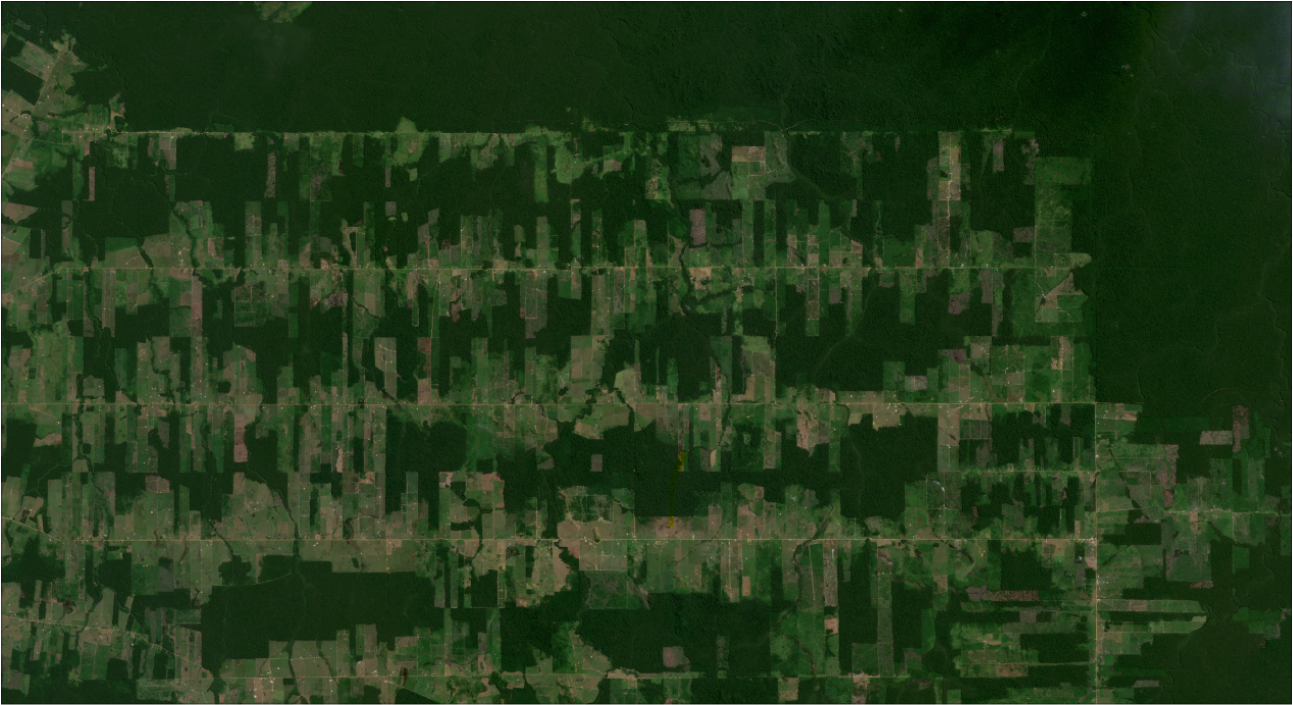
\includegraphics[width=\textwidth]{candeias_maio_2023.png}
		\caption{}
		\label{fig:candeias_maio_2023_rgb}
	\end{subfigure}
	\begin{subfigure}[b]{.8\textwidth}
		\centering
		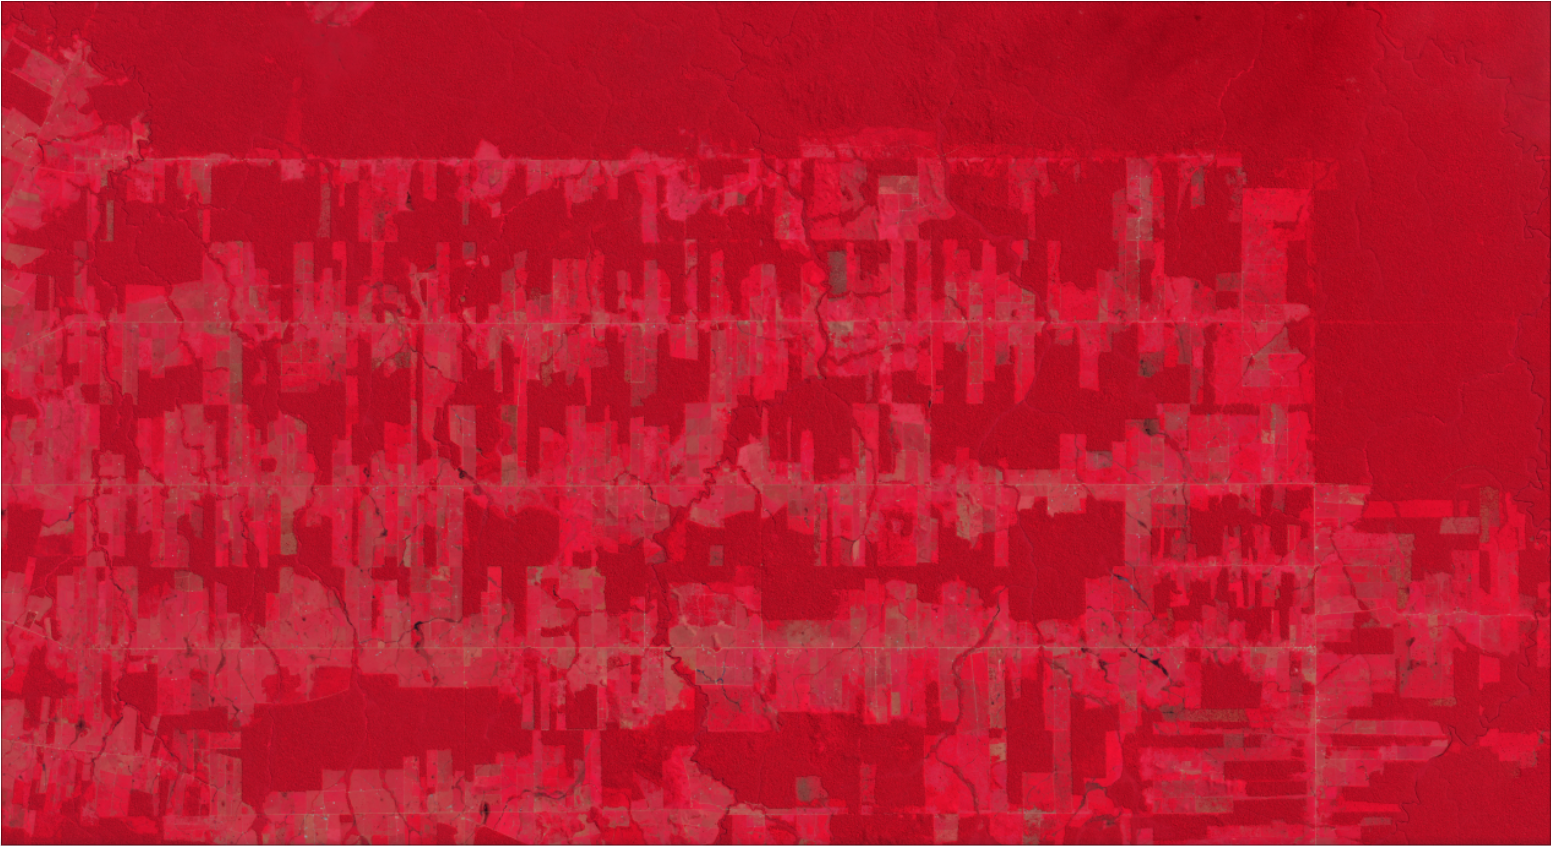
\includegraphics[width=\textwidth]{candeias_maio_2023_cir.png}
		\caption{}
		\label{fig:candeias_maio_2023_cir}
	\end{subfigure}
	
	\caption{Área de interesse em Maio de 2023 (fonte: Planet Labs PBC). \subref{fig:candeias_maio_2023_rgb} RGB. \subref{fig:candeias_maio_2023_cir} CIR.}
	\label{fig:candeias_maio_2023}
\end{figure}

Um índice comumente utilizado é o Normalized Difference Vegetation Index (NDVI), determinado pela Equação \ref{eq:ndvi}. Ao aplicar este índice em todos os pixels de uma imagem CIR, obtém-se uma imagem grayscale com escala 0-1, representada na Figura \ref{fig:candeias_maio_2023_ndvi}. Este índice baseia-se no fato da vegetação ter alta refletividade na banda NIR e baixa refletividade na banda vermelha, portanto vegetação terá índices altos \cite{eos:cir:2023}.

\begin{equation} \label{eq:ndvi}
	NDVI = \frac{NIR - RED}{NIR + RED}
\end{equation}

\begin{figure}[!htb]
	\centering
	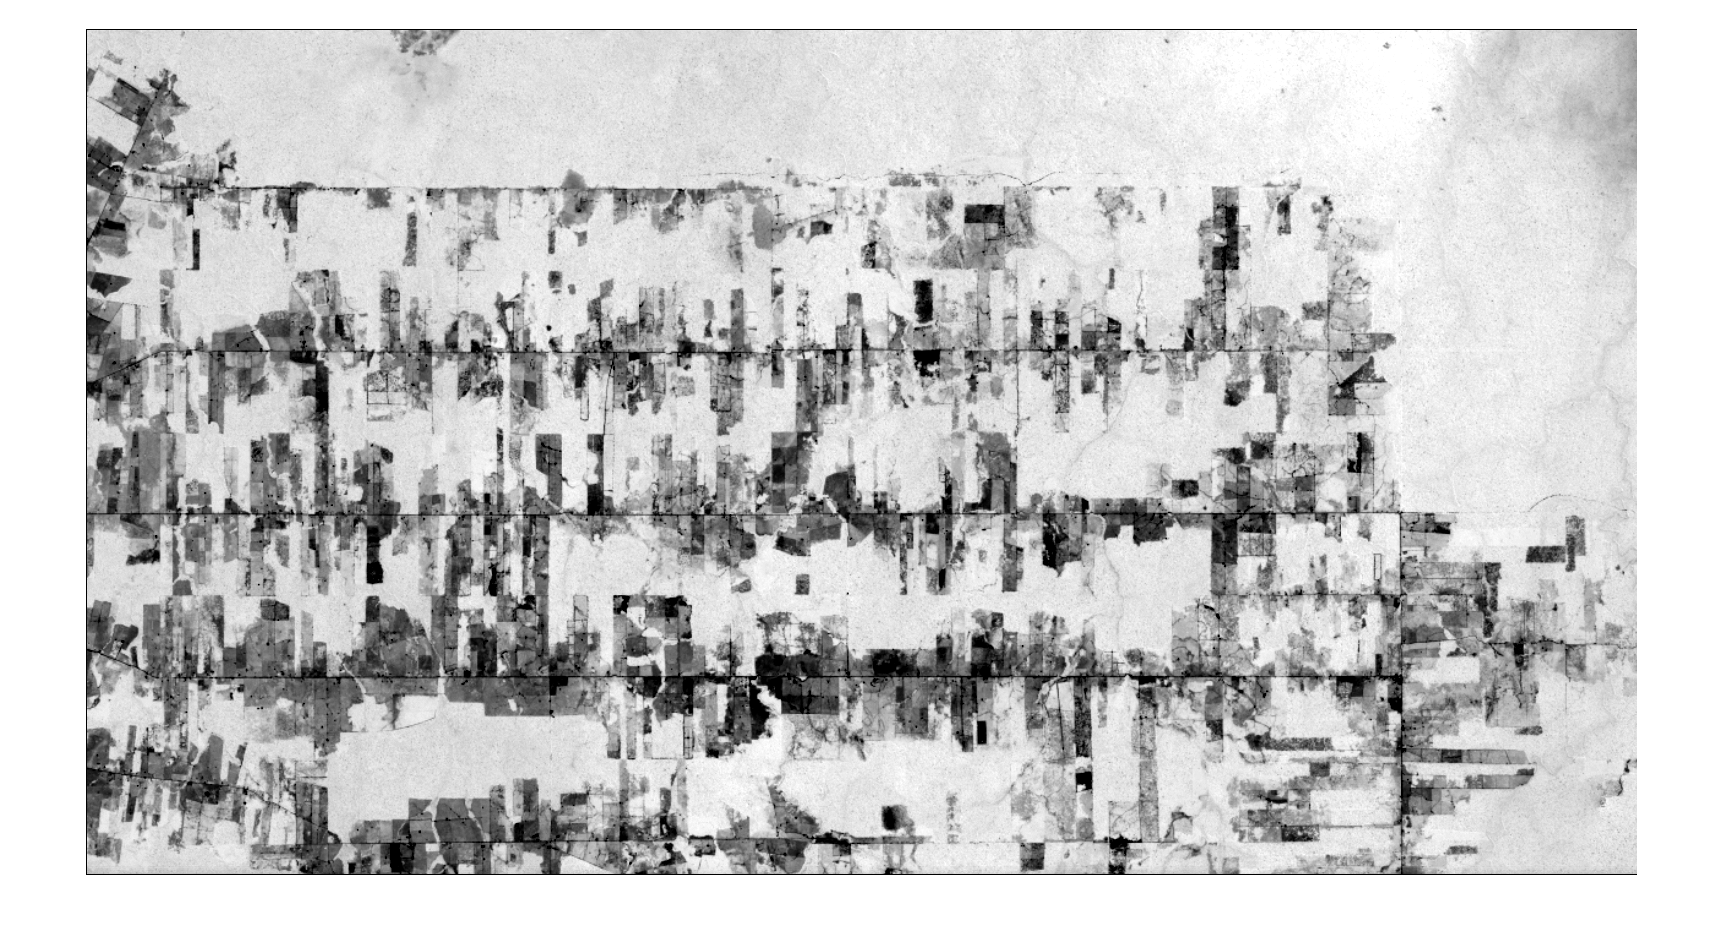
\includegraphics[width=.9\textwidth]{candeias_maio_2023_ndvi.png}
	\caption{NDVI com auto-contraste da área de interesse em Maio de 2023 (fonte: Planet Labs PBC)}
	\label{fig:candeias_maio_2023_ndvi}
\end{figure}

\subsection{Segmentação por clusterização K-Means}
\label{ss:kmeans}

O algoritmo K-Means, proposto em \cite{kmeans:1979}, divide um conjunto de pontos no espaço em K grupos (clusters), de forma que a soma quadrática das distâncias euclidianas entre pontos de um mesmo grupo seja minimizada. O algoritmo é iterativo e converge para os mínimos locais das distâncias estes clusters, ou seja, mover um ponto qualquer de um grupo para outro não diminui a soma de quadrados em nenhum dos grupos.

Em processamento digital de imagens, é utilizado para segmentação de imagens, ou seja, dividir a imagem em regiões de interesse. Sendo a coordenada dos pontos determinadas pelo nível de cinza de cada pixel, o algoritmo divide a imagem em K grupos de pixels com níveis de cinza similares \cite{dhanachandra:2015}. O mesmo princípio pode ser aplicado para imagens coloridas, onde cada ponto é representado por um vetor de 3 dimensões (RGB ou CIR).







\section{Implementação}

O programa \verb|amazonia.m| realiza o processamento de duas imagens de entrada no formato CIR, da mesma área geográfica em diferentes instantes de tempo. Aplicando duas abordagens para o algoritmo K-Means e apresentando as áreas de floresta na imagem antiga e na imagem nova, e a diferença entre elas (desmatamento/recuperação da mata).

As imagens foram obtidas dos satélites da empresa americana Planet Labs PBC. A área escolhida foi um retângulo de 1243 km\textsuperscript{2} definido pelos vértices nas coordenadas [-63.341818,-8.87654], [-62.765656,-8.87654], [-62.765656,-8.514369] e [-63.341818,-8.514369] (arquivo \verb|candeias.geojson|), um trecho do município de Candeias do Jamari, em Rondônia, Brasil. Foram escolhidos 2 \textit{basemaps} que possuem imagens CIR e que não contém nuvens na área de interesse: Junho de 2017 e Novembro de 2022. A Figura \ref{fig:candeias_imagens_cir} mostra as imagens utilizadas, retiradas de \textit{screenshots} do site da Planet Labs: \url{https://www.planet.com/explorer/?s=UNS6fwFDRaOTUSdpRXroiQ}

\begin{figure}[!htb]
	\centering
	\begin{subfigure}[b]{.45\textwidth}
		\centering
		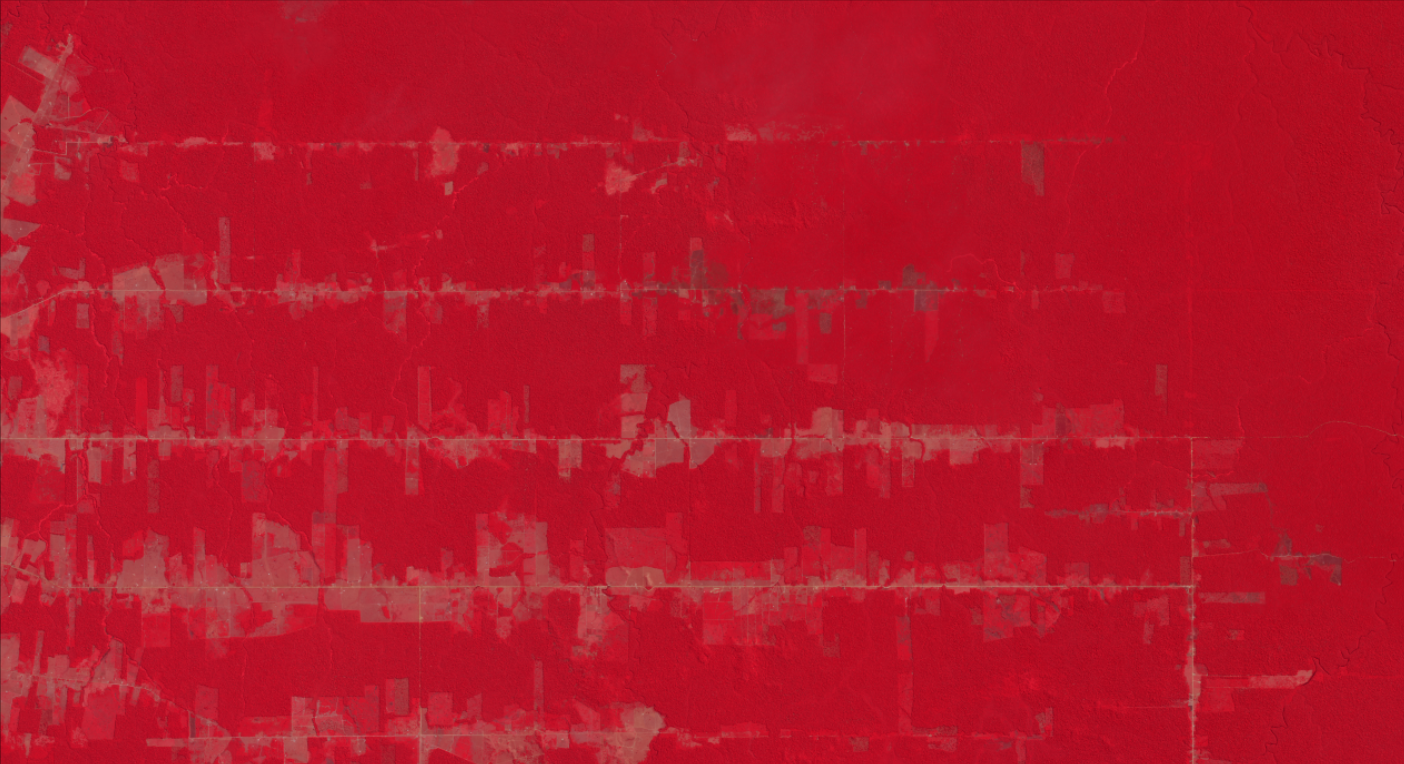
\includegraphics[width=\textwidth]{candeias_junho_2017_cir.png}
		\caption{}
		\label{fig:candeias_junho_2017_cir}
	\end{subfigure}
	\begin{subfigure}[b]{.45\textwidth}
		\centering
		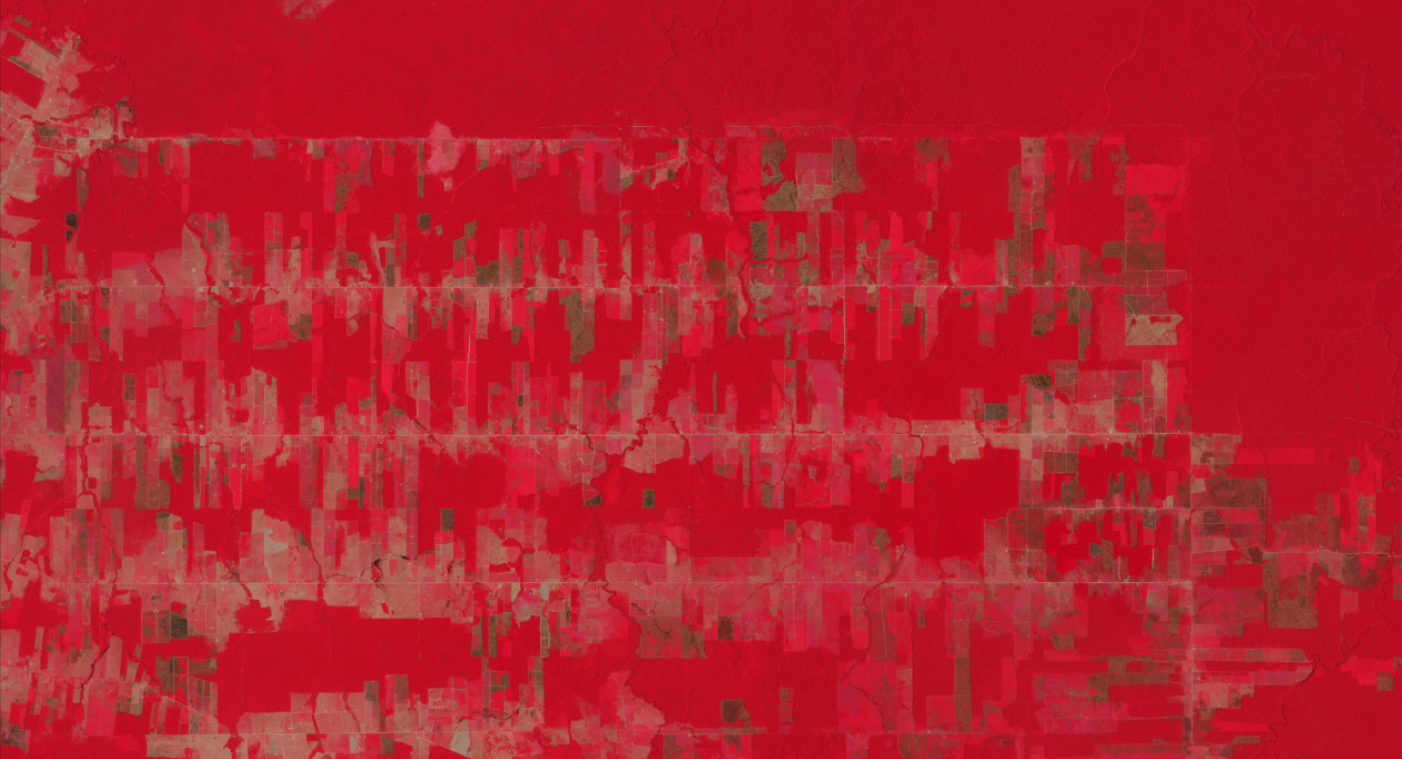
\includegraphics[width=\textwidth]{candeias_nov_2022_cir.png}
		\caption{}
		\label{fig:candeias_nov_2022_cir}
	\end{subfigure}
	
	\caption{Área de interesse (fonte: Planet Labs PBC). \subref{fig:candeias_junho_2017_cir} Junho de 2017. \subref{fig:candeias_nov_2022_cir} Novembro de 2022.}
	\label{fig:candeias_imagens_cir}
\end{figure}

O algoritmo foi implementado em MATLAB em duas abordagens: Primeiro, a função \verb|process_image_ndvi.m| utiliza o índice NDVI que considera apenas os canais NIR e RED. Segundo, a função \verb|process_image_cir.m| utiliza os 3 os canais da imagem CIR.

O pré-processamento da imagem consiste em: Auto-contraste utilizando a função \verb|imadjust| do MATLAB, para melhorar a visualização; e aplicação de um filtro passa-baixa gaussiano de tamanho 6, sigma de 0.8.

Para o tratamento da imagem CIR completa, foi optado por não realizar auto-contraste na camada NIR, pois observou-se um aumento considerável de ruídos e degradação na segmentação. A Figura \ref{fig:candeias_maio_2023_cir_contrast} mostra uma imagem CIR com auto-contraste apenas na camada RED e GREEN.

\begin{figure}[!htb]
	\centering
	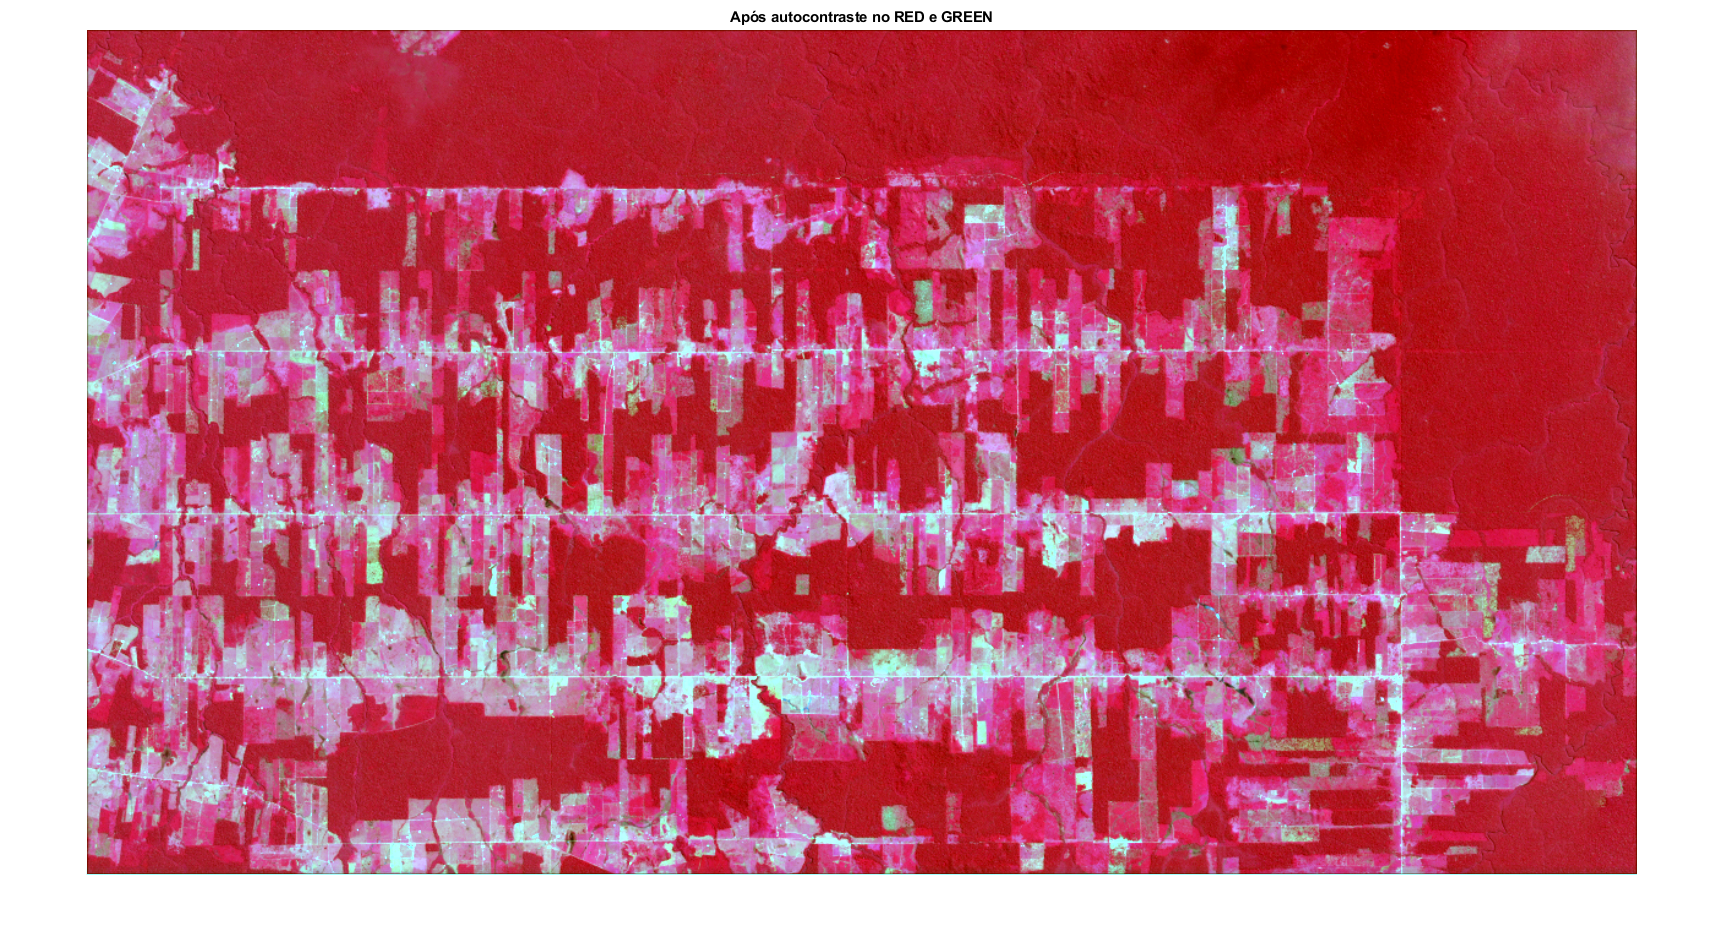
\includegraphics[width=.9\textwidth]{candeias_maio_2023_cir_contrast.png}
	\caption{Imagem CIR com auto-contraste nas camadas RED e GREEN da área de interesse em Maio de 2023 (fonte: Planet Labs PBC)}
	\label{fig:candeias_maio_2023_cir_contrast}
\end{figure}
O processamento da imagem é feito pelo algoritmo de clusterização K-Means com K=3. Este K foi determinado empiricamente de forma que uma das segmentações contenha vegetação (floresta), e as outras contenham 2 níveis de vegetação degradada. A Figura \ref{fig:candeias_maio_2023_ndvi_clusters} mostra os clusters retirados de uma imagem NDVI.

\begin{figure}[!htb]
	\centering
	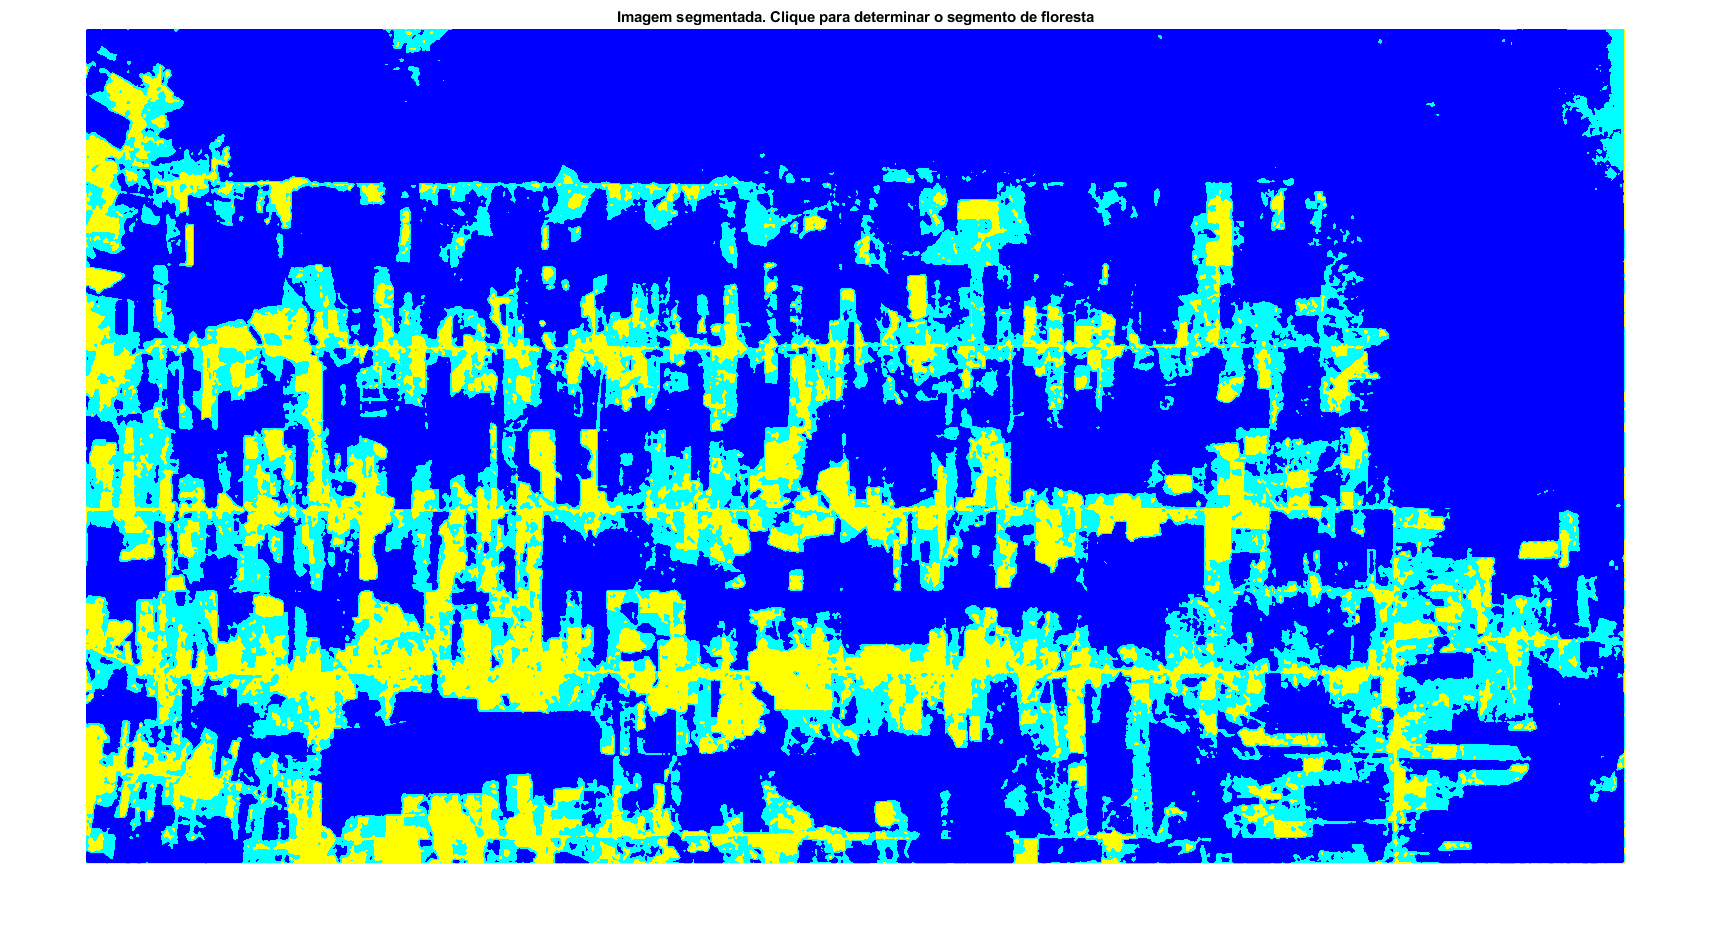
\includegraphics[width=.9\textwidth]{candeias_maio_2023_ndvi_clusters.png}
	\caption{Clusters da imagem NDVI da área de interesse em Maio de 2023 (fonte: Planet Labs PBC)}
	\label{fig:candeias_maio_2023_ndvi_clusters}
\end{figure}

O usuário deve selecionar com o mouse qual das regiões segmentadas é a floresta, e o algoritmo determina a área de floresta preservada como o número de pixels desta região, multiplicada pela área correspondente de um pixel. A área de floresta degradada é determinada como a diferença entre a área total e a área de floresta.

\section{Resultados e conclusões}

Os dados obtidos da comparação das imagens de Junho de 2017 e Novembro de 2022, através das duas técnicas de processamento são mostrados abaixo:

\begin{verbatim}
================ NDVI ================
Área analisada = 1.2430 km^2 	(100.00%)
--------------------------------------
Floresta
--------------------------------------
Antigo  : Área = 0.9838 km^2 	(79.15%)
Novo    : Área = 0.7416 km^2 	(59.66%)
Diff    : Área = -0.2422 km^2 	(-19.49%)

================ CIR =================
Área analisada = 1.2430 km^2 	(100.00%)
--------------------------------------
Floresta
--------------------------------------
Antigo  : Área = 0.9787 km^2 	(78.74%)
Novo    : Área = 0.7342 km^2 	(59.07%)
Diff    : Área = -0.2446 km^2 	(-19.67%)
\end{verbatim}

É possível observar que ambos obtém resultados bem similares, com uma diferença máxima de 0.59\% entre técnicas. A diferença de área de floresta degradada é de 0.18\%, o que é considerado insignificante.

Uma análise visual das segmentações obtidas nos métodos NDVI e CIR (Figura \ref{fig:candeias_nov_2022_overlay}) indica a existência de falsos-positivos em ambos os casos, ou seja, áreas desmatadas que não foram identificadas pelo algoritmo.

\begin{figure}[!htb]
	\centering
	\begin{subfigure}[b]{\textwidth}
		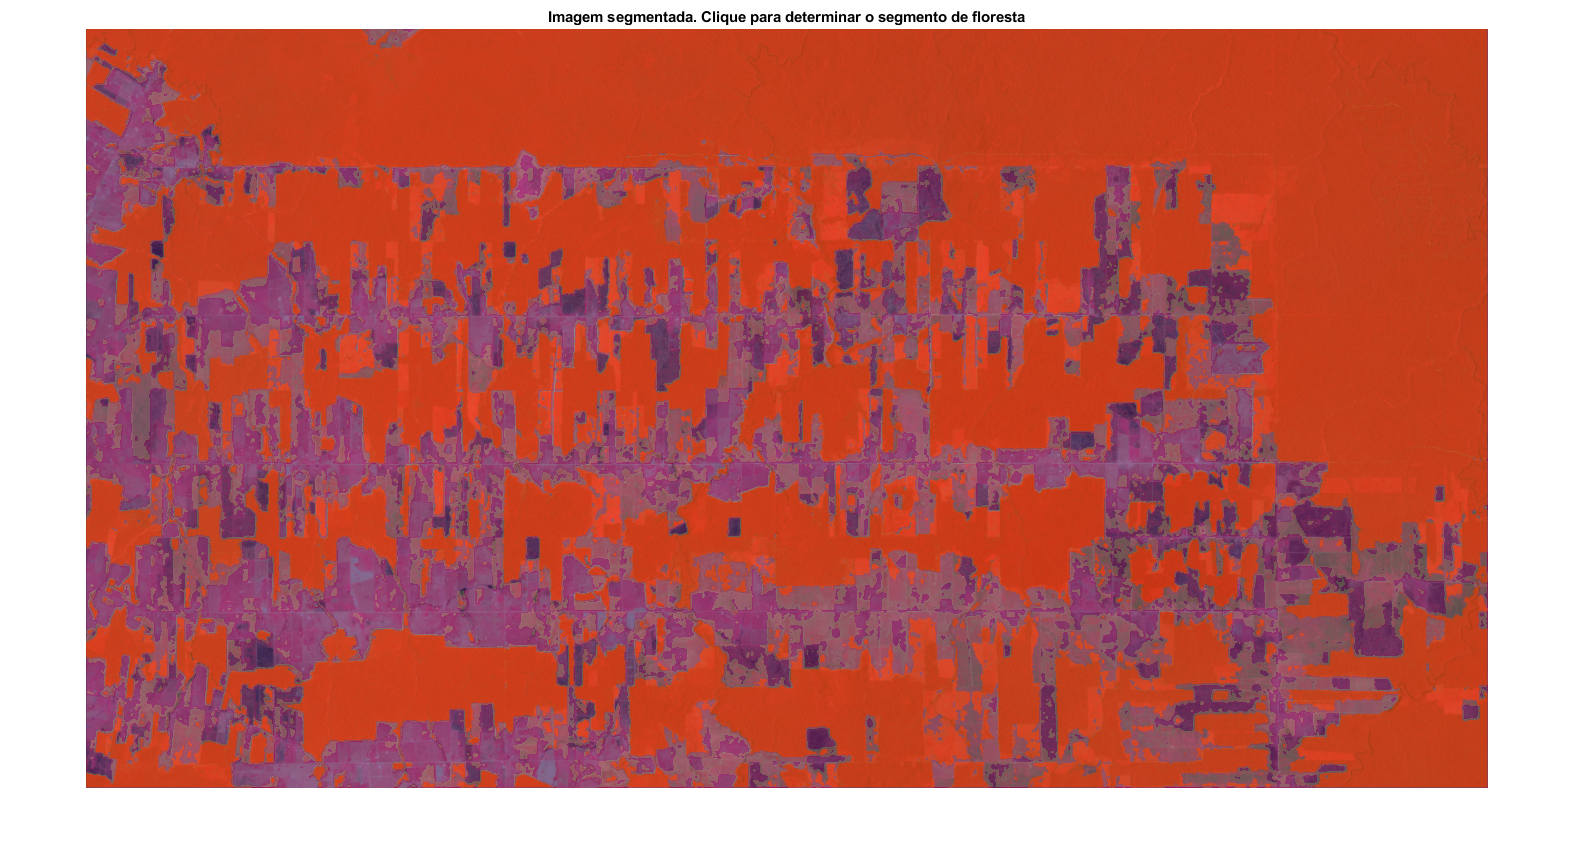
\includegraphics[width=\textwidth]{candeias_nov_2022_ndvi_overlay.png}
		\caption{}
		\label{fig:candeias_nov_2022_ndvi_overlay}
	\end{subfigure}
	\begin{subfigure}[b]{\textwidth}
		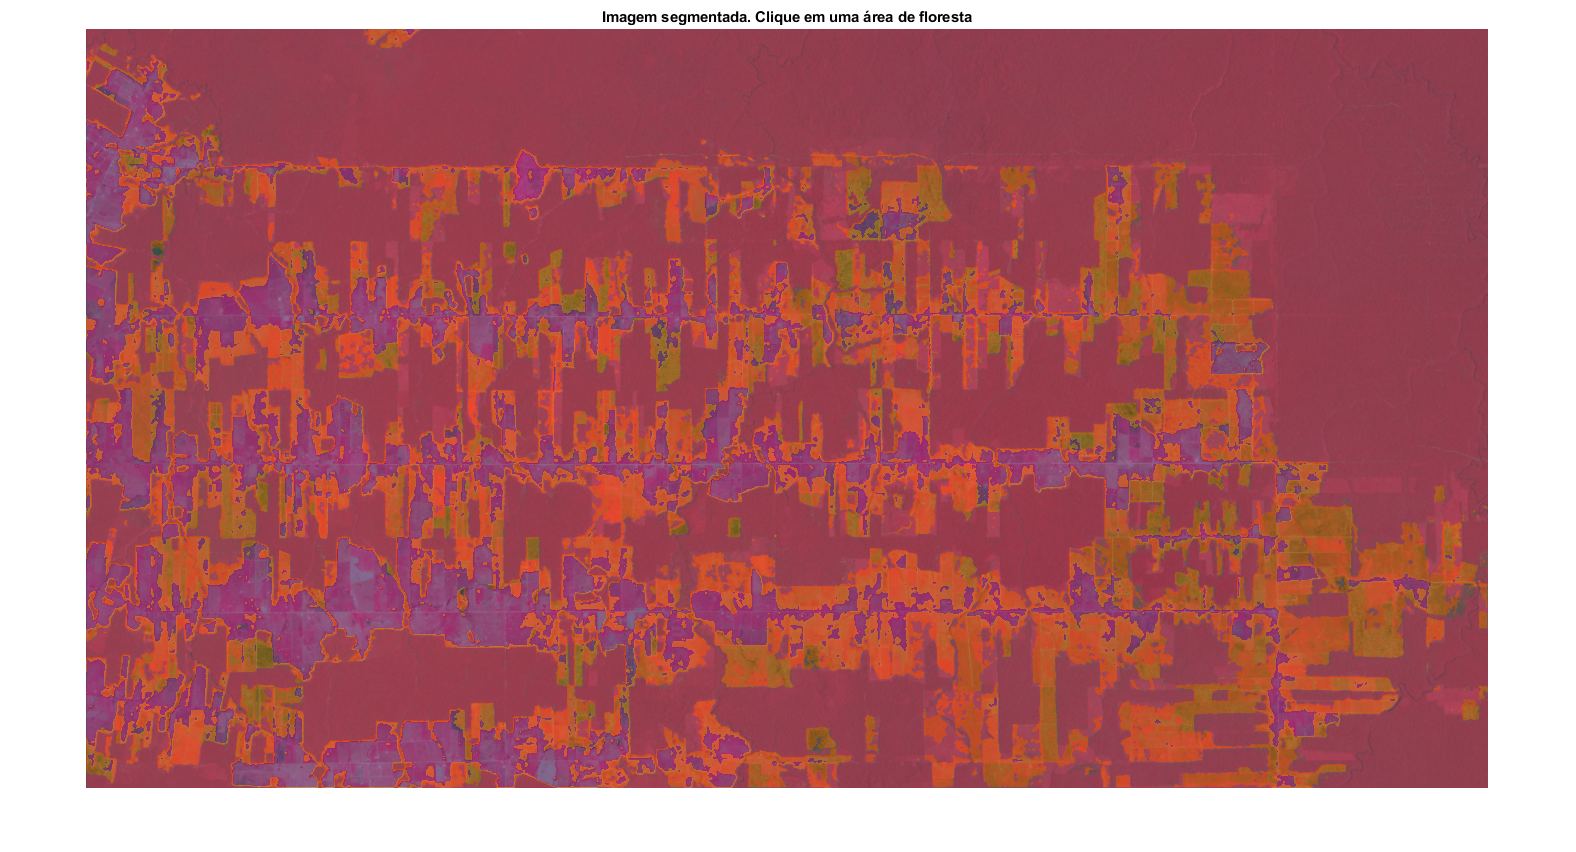
\includegraphics[width=\textwidth]{candeias_nov_2022_cir_overlay.png}
		\caption{}
		\label{fig:candeias_nov_2022_cir_overlay}
	\end{subfigure}
	
	\caption{Segmentação das imagens \subref{fig:candeias_nov_2022_ndvi_overlay} NDVI e \subref{fig:candeias_nov_2022_cir_overlay} CIR}
	\label{fig:candeias_nov_2022_overlay}
\end{figure}


Futuros trabalhos devem buscar imagens de maiores áreas geográficas, maior resolução, imagens de diferentes satélites e instantes de tempo. É interessante automatizar a seleção da região de floresta, e comparar os resultados com outras técnicas de clusterização, como o K-NN, e algoritmos utilizados pelo INPE.

É relevante a comparação com os mapas e estatísticas oficiais do INPE, disponibilizados na ferramenta TerraBrasilis e manipuláveis pelo Sistema de Informação Geográfica (SIG) TerraView, do INPE. Estas ferramentas foram investigadas para este projeto, porém não foi possível obter resultados satisfatórios para comparação devido à complexidade de manipulação dos programas necessários.


% Referências Bibliográficas %
% usar 'cite'  %
\bibliography{bibliografia}
\bibliographystyle{plain}

\end{document}
% fim do documento